\documentclass[9pt]{beamer}
\mode<presentation>

% Theme choice:
\usetheme{Madrid}%Darmstadt 

\usecolortheme[RGB={0,100,50}]{structure}
 \usefonttheme{structurebold} 
\setbeamercovered{invisible}
%\setbeamertemplate{navigation symbols}{}
\usepackage{dynblocks}
\usepackage{textpos}
\usepackage{amsfonts}
\usepackage{amsmath}
\usepackage{amssymb}
\usepackage{amsthm}
\usepackage{tikz}
\usepackage{pgfplots}
\pgfplotsset{compat=1.18}
\newtheorem{teorema}{Teorema}\usepackage{mathtools}
\renewcommand{\proofname}{Prova}
\usepackage[portuguese]{babel}

\uselanguage{Portuguese}
\languagepath{Portuguese}

\deftranslation[to=Portuguese]{Theorem}{Teorema}
\deftranslation[to=Portuguese]{Lemma}{Lema}
\deftranslation[to=Portuguese]{Corollary}{Corolário}
\deftranslation[to=Portuguese]{Proof}{Prova}

\usepackage{dutchcal}
\usepackage{hyperref}
\usepackage[utf8]{inputenc}
\usepackage[T1]{fontenc}
\usepackage{amsthm}


\usepackage[affil-it]{authblk} 
\usepackage{etoolbox}
\usepackage{lmodern}

\makeatletter
\patchcmd{\@maketitle}{\LARGE \@title}{\fontsize{18}{19.2}\selectfont\@title}{}{}
\makeatother

\renewcommand\Authfont{\fontsize{12}{14.4}\selectfont}
\renewcommand\Affilfont{\fontsize{9}{10.8}\itshape}

% Title page details: 
\title[Presentation]{ENGENHARIA DA QUALIDADE E CONFIABILIDADE} %add title


\institute[UniRV]{\textbf{\large  \textcolor{structure}{\textbf{\large
Google SRE, conceito de DEV e OPS, diferenças entre SRE e DevOPs
}} %add name 
% \hspace{0.5pt}
\\ \qquad
\\Professor: Me. Sergio Souza Novak 
\\Faculdade de Engenharia de Software}
} 
% \titlegraphic{\includegraphics[width=5cm]{msu.eps}}
\titlegraphic{
\includegraphics[width=5cm]{Universidade_de_Rio_Verde.jpg}}
\date{}

% Logo only on title page
%\logo{
\includegraphics[width=1cm,keepaspectratio]{Logo.png}}
\usepackage[pscoord]{eso-pic}


\begin{document}

% Title page frame
%\begin{frame}
    %\titlepage 
%\end{frame}
\frame[plain]{\titlepage}
%logo
\AddToShipoutPictureFG{
    \put(\LenToUnit{.92\paperwidth},
    \LenToUnit{.185\paperheight})
    {\vtop{{\null}
    \makebox{
\includegraphics[width=.8cm,keepaspectratio]{Universidade_de_Rio_Verde.jpg}}}}}


\begin{frame}{Sumário}
  \tableofcontents
\end{frame}
\section{O que é a engenharia de confiabilidade}
% Slide 1: Introdução a Fermat
\begin{frame}{Introdução à Engenharia da Qualidade}

\begin{itemize}
    \item A \textbf{Engenharia da Qualidade} é a área da engenharia dedicada ao
    planejamento, controle, garantia e melhoria da qualidade de produtos e processos.
    
    \item Seu foco principal é \textbf{atender e superar as expectativas do cliente},
    assegurando conformidade com requisitos técnicos, normas e especificações.
    
    \item Utiliza métodos estatísticos, ferramentas da qualidade e abordagens
    sistemáticas para \textbf{redução de falhas, desperdícios e variabilidade}.
\end{itemize}

\end{frame}



\begin{frame}{Áreas da Engenharia da Qualidade}

\begin{itemize}
    \item Está presente em diversos setores:
    \begin{itemize}
        \item Indústria
        \item Serviços
        \item Agronegócio
        \item Tecnologia da Informação
    \end{itemize}

    \item Contribuições principais:
    \begin{itemize}
        \item Aumento da confiabilidade
        \item Redução de custos
        \item Melhoria contínua
        \item Competitividade organizacional
    \end{itemize}
\end{itemize}

\end{frame}
\section{Livros utilizados na disciplina}
\begin{frame}{Livros utilizados na disciplina}

\begin{figure}
\centering
\begin{minipage}{0.25\textwidth}
    \centering
    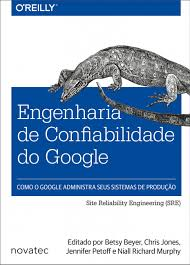
\includegraphics[width=\textwidth]{eng_conf_google.jpeg}
    \caption{Site Reliability Engineering — Google}
\end{minipage}
% \hfill
\begin{minipage}{0.25\textwidth}
    \centering
    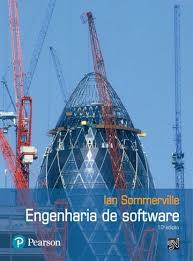
\includegraphics[width=\textwidth]{sommerville.jpeg}
    \caption{Software Engineering — Ian Sommerville}
\end{minipage}
\end{figure}
\end{frame}
\section{Formas de avaliação}

\begin{frame}{Forma de Avaliação}

A avaliação da disciplina será composta por três notas:

\begin{itemize}
  \item \textbf{N1} – Média das atividades realizadas aos sábados;
  \item \textbf{N2} – Média das atividades realizadas aos sábados;
  \item \textbf{N3} – Média das atividades realizadas aos sábados.
\end{itemize}

\vspace{0.4cm}

Cada nota corresponderá exclusivamente ao desempenho do aluno nas atividades desenvolvidas durante os encontros de sábado.
A Nota Final é obviamente a média aritmética simples das três notas:
\end{frame}
\section{O programa apollo e a engenharia de confiabilidade}

\begin{frame}{Margaret Hamilton e o Programa Apollo}

\begin{figure}
    \centering
    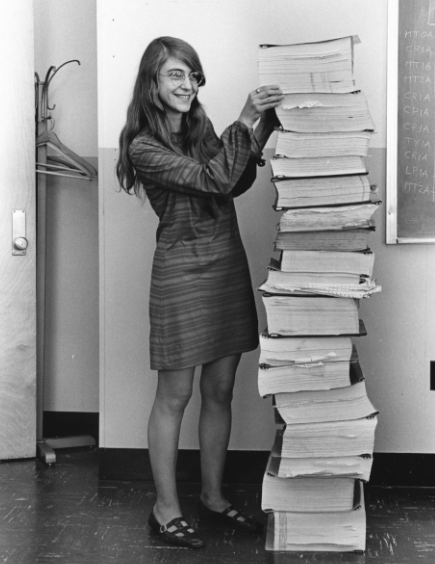
\includegraphics[width=0.25\textwidth]{margaret.png}
    \caption{Margaret Hamilton no Laboratório de Instrumentação do MIT}
\end{figure}

Margaret Hamilton foi engenheira de software no MIT e atuou no desenvolvimento
do software do programa Apollo da NASA. Seu trabalho pioneiro em
\textbf{engenharia de software}, especialmente no tratamento de falhas críticas,
é frequentemente citado como um precursor das práticas modernas de
\textbf{Site Reliability Engineering (SRE)}.

\begin{itemize}
  \item Ênfase em confiabilidade e tolerância a falhas;
  \item Desenvolvimento de software rigorosamente engenheirado;
  \item Antecipação e tratamento de falhas raras, porém catastróficas.
\end{itemize}

\end{frame}

\begin{frame}{O Episódio no Simulador de Missão}
\begin{figure}
    \centering
    
\includegraphics[width=0.25\textwidth]{filha.jpeg}
    \caption{DSKY do computador Apollo}
\end{figure}
Durante testes no computador híbrido de simulação do Apollo, Margaret levou sua
filha Lauren ao trabalho.

\begin{itemize}
  \item Lauren pressionou teclas do DSKY de forma aleatória;
  \item Isso provocou a falha de uma missão simulada;
  \item Revelou um comportamento inesperado do sistema.
\end{itemize}

O episódio expôs um risco que não havia sido considerado pela equipe.
\end{frame}
\begin{frame}{O Problema Técnico Identificado}

A falha ocorreu ao selecionar inadvertidamente o programa \textbf{P01}:

\begin{itemize}
  \item O P01 limpava os dados de navegação;
  \item Sem esses dados, o computador não conseguia pilotar a nave;
  \item Em uma missão real, isso impediria o retorno à Terra.
\end{itemize}

Tratava-se de um erro humano simples com consequências catastróficas.
\end{frame}
\begin{frame}{A Proposta de Margaret Hamilton}
\begin{figure}
    \centering
    
\includegraphics[width=0.25\textwidth]{erros_verificacao.png}
    \caption{Proposta de solução de Margaret Hamilton}
\end{figure}
Com mentalidade de SRE, Margaret propôs:

\begin{itemize}
  \item Inclusão de um código de verificação de erro;
  \item Detecção e bloqueio da execução do P01 durante o voo;
  \item Mecanismo de recuperação automática.
\end{itemize}

A proposta foi rejeitada sob o argumento de que os astronautas
\textit{“não cometeriam erros”}.
\end{frame}
\begin{frame}{O Incidente na Apollo 8}
\begin{figure}
    \centering
    
\includegraphics[width=0.25\textwidth]{jim_lovell.png}
    \caption{Jim Lovell durante a missão Apollo 8}
\end{figure}
Poucos dias depois, durante a missão Apollo 8:

\begin{itemize}
  \item O astronauta Jim Lovell selecionou o P01 por engano;
  \item Os dados de navegação foram apagados;
  \item A missão correu sério risco de fracasso.
\end{itemize}

Graças à documentação atualizada, foi possível recuperar os dados
e salvar a missão.
\end{frame}
\begin{frame}{Lições para Engenharia e SRE}

O episódio evidencia princípios centrais do pensamento SRE:

\begin{itemize}
  \item Erros humanos são inevitáveis;
  \item Sistemas críticos devem ser resilientes a esses erros;
  \item Documentação, preparação e engenharia preventiva salvam sistemas;
  \item Confiabilidade deve ser tratada como requisito de projeto.
\end{itemize}

Essas lições continuam diretamente relevantes para sistemas modernos.
\end{frame}
\section{O método sysadmin (operação) e desenvolvimento}

\begin{frame}{Abordagem Tradicional com Administradores de Sistemas}
\begin{figure}
\centering
\begin{minipage}{0.25\textwidth}
    \centering
    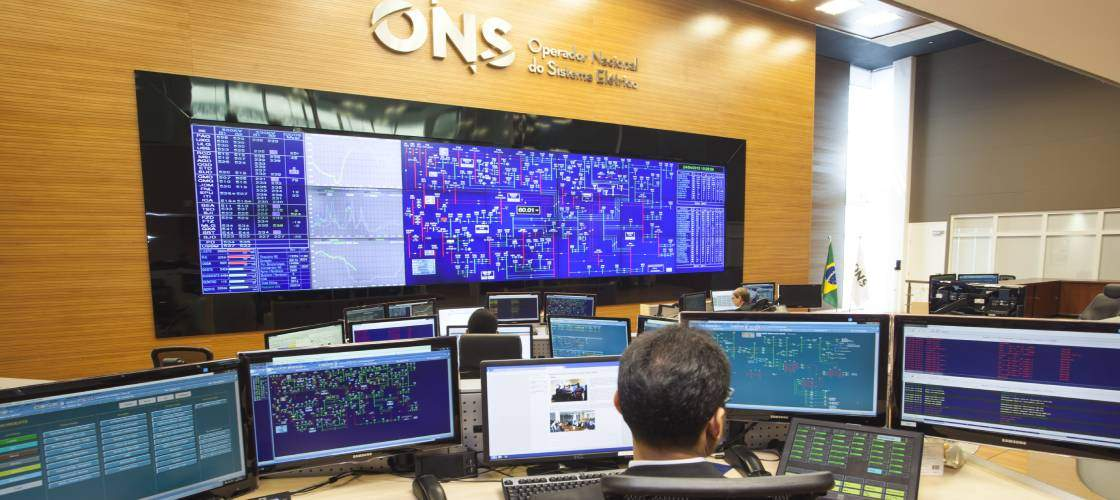
\includegraphics[width=\textwidth]{operador_de_sistema.jpg}
    \caption{Operador de Sistema ou Sysadmin}
\end{minipage}
% \hfill
\begin{minipage}{0.25\textwidth}
    \centering
    
\includegraphics[width=\textwidth]{dev.jpeg}
    \caption{Desenvolvedor}
\end{minipage}
\end{figure}
Historicamente, as organizações têm utilizado \textbf{administradores de sistemas (sysadmins)}
para operar sistemas computacionais complexos e prover serviços.

\begin{itemize}
  \item Integração de componentes de software existentes;
  \item Implantação e operação de serviços em produção;
  \item Resposta a eventos, falhas e atualizações;
  \item Crescimento da equipe conforme aumentam a complexidade e o tráfego.
\end{itemize}

Com o tempo, consolidou-se a separação entre as equipes de
\textbf{Desenvolvimento (Dev)} e \textbf{Operações (Ops)}, cada uma com
habilidades e responsabilidades distintas.

\end{frame}
\begin{frame}{Vantagens da Abordagem com Sysadmins}

O modelo tradicional de gerenciamento de serviços apresenta vantagens
importantes para as organizações:

\begin{itemize}
  \item Paradigma amplamente conhecido e adotado no mercado;
  \item Facilidade de implementação organizacional;
  \item Grande disponibilidade de profissionais especializados;
  \item Existência de ferramentas, softwares e soluções consolidadas;
  \item Redução da necessidade de projetar sistemas do zero.
\end{itemize}

Essa abordagem permitiu, por muitos anos, a operação eficiente de serviços
em diferentes contextos organizacionais.

\end{frame}
\begin{frame}{Desvantagens e Conflitos no Modelo Dev/Ops}

Apesar das vantagens, o modelo apresenta limitações relevantes:

\textbf{Custos diretos}
\begin{itemize}
  \item Forte dependência de intervenção manual;
  \item Crescimento linear do custo operacional com o aumento do serviço;
  \item Necessidade constante de ampliação da equipe.
\end{itemize}

\textbf{Custos indiretos}
\begin{itemize}
  \item Diferenças de cultura, linguagem e incentivos entre Dev e Ops;
  \item Conflitos sobre risco, estabilidade e velocidade de entrega;
  \item Tensão entre lançar novas funcionalidades e manter a confiabilidade.
\end{itemize}

Esses conflitos estruturais motivaram o surgimento de abordagens modernas,
como \textbf{DevOps} e \textbf{Site Reliability Engineering (SRE)}.

\end{frame} 
\begin{frame}{Preocupações da Equipe de Desenvolvimento}
\begin{figure}
    \centering
    
\includegraphics[width=0.25\textwidth]{dev.jpeg}
    \caption{O desenvolvedor quer ver os clientes usando o produto.}
\end{figure}
A equipe de \textbf{Desenvolvimento} tem como objetivo central a evolução
do produto e sua adoção pelos usuários.

\begin{itemize}
  \item Lançar novas funcionalidades com rapidez;
  \item Responder rapidamente a demandas do mercado;
  \item Introduzir mudanças frequentes no sistema;
  \item Valorizar inovação e velocidade de entrega.
\end{itemize}

Do ponto de vista do desenvolvimento, mudanças são essenciais para
o progresso e a competitividade do serviço.

\end{frame}
\begin{frame}{Preocupações da Equipe de Operações}
\begin{figure}
    \centering
    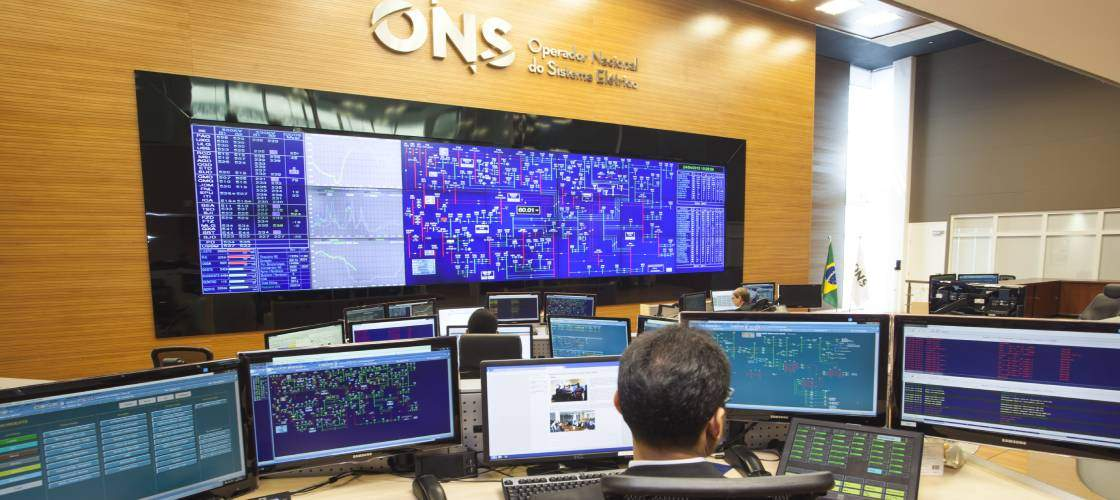
\includegraphics[width=0.5\textwidth]{operador_de_sistema.jpg}
    \caption{O operador quer manter o serviço funcionando.}
\end{figure}
A equipe de \textbf{Operações (Ops)} tem como foco principal a
\textbf{estabilidade e confiabilidade} do serviço em produção.

\begin{itemize}
  \item Manter o sistema funcionando continuamente;
  \item Minimizar falhas e interrupções de serviço;
  \item Reduzir riscos associados a mudanças;
  \item Proteger o ambiente de produção.
\end{itemize}

Como grande parte das falhas decorre de mudanças, a equipe de operações
tende a ser naturalmente avessa a elas.

\end{frame}
\begin{frame}{Conflito Implícito entre Desenvolvimento e Operações}
\begin{figure}
    \centering
    
\includegraphics[width=0.5\textwidth]{conflito.jpeg}
    \caption{Briga na daily entre Dev e Ops.}
\end{figure}
Embora ambos os grupos reconheçam posições extremas como inaceitáveis,
seus interesses entram em conflito na prática.

\begin{itemize}
  \item Desenvolvimento não pode lançar tudo sem restrições;
  \item Operações não pode impedir qualquer mudança;
  \item Diferenças de vocabulário e percepção de risco dificultam o diálogo.
\end{itemize}

Esse desalinhamento leva frequentemente a conflitos organizacionais
silenciosos, porém persistentes.

\end{frame}
\begin{frame}{A Guerra de Trincheiras entre Dev e Ops}

Diante da dificuldade de explicitar interesses, as equipes recorrem
a estratégias defensivas.

\begin{itemize}
  \item Comunicação indireta e reativa;
  \item Tentativas de impor controles ao invés de cooperação;
  \item Falta de confiança mútua ao longo do tempo.
\end{itemize}

Esse cenário caracteriza uma verdadeira \textbf{guerra de trincheiras},
onde cada grupo tenta proteger seus objetivos.

\end{frame}
\begin{frame}{Gates e Barreiras Impostos por Operações}
\begin{figure}
    \centering
    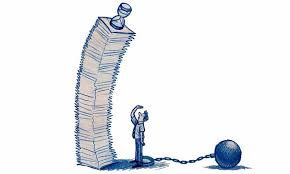
\includegraphics[width=0.4\textwidth]{burocracia.jpeg}
    \caption{Desenvolvedor sofrendo com burocracia.}
\end{figure}
Para reduzir riscos, a equipe de operações introduz
\textbf{pontos de verificação (gates)} antes de lançamentos.

\begin{itemize}
  \item Revisões extensas de mudanças;
  \item Verificação de falhas históricas;
  \item Listas longas de requisitos para aprovação;
  \item Adoção de critérios nem sempre proporcionais ao risco.
\end{itemize}

Embora bem-intencionadas, essas práticas aumentam a fricção
no processo de entrega.

\end{frame}
\begin{frame}{Menos Lançamentos Formais}
\begin{figure}
    \centering
    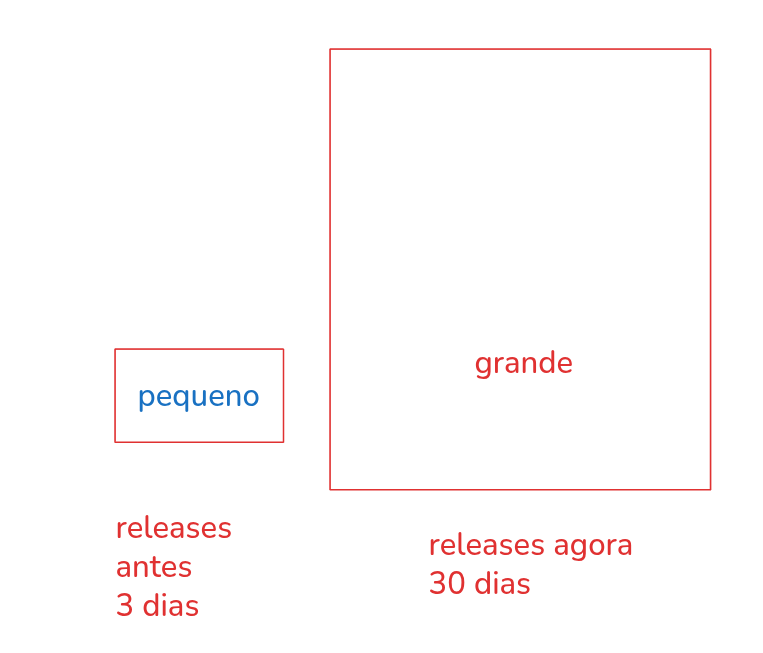
\includegraphics[width=0.4\textwidth]{releases.png}
    \caption{Visão geral das entregas.}
\end{figure}
Diante de processos de aprovação longos e rigorosos, a equipe de
desenvolvimento reduz a frequência de lançamentos formais.

\begin{itemize}
  \item Consolidação de várias mudanças em um único release;
  \item Redução do custo burocrático por implantação;
  \item Aumento do tamanho e do risco de cada lançamento.
\end{itemize}

Essa prática diminui a exposição a revisões frequentes, mas dificulta
a identificação da causa de falhas em produção.
\end{frame}
\begin{frame}{Feature Flags e Atualizações Incrementais}

Para evitar novos ciclos de aprovação, os desenvolvedores utilizam
mecanismos que permitem alterar o comportamento do sistema sem
realizar um novo deploy.

\begin{itemize}
  \item Uso de \textbf{feature flags} para ativar ou desativar funcionalidades;
  \item Aplicação de \textit{cherry-picks} e correções pontuais;
  \item Mudanças graduais com impacto aparentemente reduzido.
\end{itemize}

Essas técnicas aumentam a flexibilidade, porém introduzem maior
complexidade lógica e dependência de configurações.
\end{frame}
\begin{frame}{Divisão do Produto e Aumento da Complexidade}

Outra resposta comum é a divisão do sistema em partes menores,
limitando o escopo das revisões de lançamento.

\begin{itemize}
  \item Separação em módulos ou serviços;
  \item Revisões focadas em componentes isolados;
  \item Redução aparente do risco por mudança.
\end{itemize}

Apesar dos benefícios organizacionais, essa fragmentação pode gerar
complexidade operacional e falhas emergentes na integração.
\end{frame}

\begin{frame}{A Abordagem do Google para Gerenciamento de Serviços}
\begin{figure}
    \centering
    
\includegraphics[width=0.4\textwidth]{google.png}
    \caption{O Google é pioneiro em SRE.}
\end{figure}

O Google parte do princípio de que o conflito entre
\textbf{desenvolvimento e operações não é inevitável}.

\begin{itemize}
  \item O modelo tradicional de sysadmins gera conflitos estruturais;
  \item Grande dependência de intervenção manual;
  \item Dificuldade de escalar serviços confiáveis.
\end{itemize}

Para resolver esse problema, o Google adotou uma abordagem distinta:
\textbf{Site Reliability Engineering (SRE)}.

\end{frame}
\begin{frame}{O que é Site Reliability Engineering (SRE)?}

Segundo a definição clássica do Google:

\begin{block}{Definição}
SRE é o que acontece quando você pede a um engenheiro de software
para projetar uma equipe de operações.
\end{block}

\begin{itemize}
  \item Operações tratadas como um problema de engenharia;
  \item Uso intensivo de software para gerenciar serviços;
  \item Substituição de tarefas manuais por automação.
\end{itemize}

\end{frame}
\begin{frame}{Composição das Equipes de SRE}

As equipes de SRE do Google são formadas por profissionais com forte
base em engenharia de software.

\begin{itemize}
  \item 50–60\%: Engenheiros de Software contratados pelo processo padrão;
  \item 40–50\%: Profissionais com perfil quase equivalente a engenheiros
  de software (85–99\% das habilidades exigidas);
  \item Conhecimentos adicionais valorizados:
  \begin{itemize}
    \item Sistemas Unix;
    \item Redes (Camadas 1 a 3).
  \end{itemize}
\end{itemize}

\end{frame}
\begin{frame}{Cultura e Perfil dos SREs}

Todos os SREs compartilham uma característica fundamental:
\textbf{resolver problemas complexos por meio de software}.

\begin{itemize}
  \item Baixa tolerância a tarefas manuais repetitivas;
  \item Forte capacidade de projetar e implementar automações;
  \item Formação técnica próxima à dos desenvolvedores;
  \item Integração cultural com equipes de produto.
\end{itemize}

Essa diversidade de experiências resulta em sistemas mais robustos
e bem projetados.

\end{frame}
\begin{frame}{Engenharia como Base da Escalabilidade}

Na abordagem SRE, \textbf{engenharia constante é essencial}.

\begin{itemize}
  \item Sem automação, a carga operacional cresce continuamente;
  \item Modelos tradicionais escalam de forma linear:
  mais tráfego → mais pessoas;
  \item SRE busca escalar serviços por meio de software,
  não por aumento de equipes.
\end{itemize}

O objetivo é que sistemas bem-sucedidos não exijam crescimento
proporcional da equipe de operações.

\end{frame}
\begin{frame}{Automação vs. Tempo de Operação}

\begin{figure}
\centering
\begin{tikzpicture}
\begin{axis}[
    width=0.85\textwidth,
    height=0.5\textwidth,
    xlabel={Tempo},
    ylabel={Carga de Operações Manuais},
    xmin=0, xmax=10,
    ymin=0, ymax=10,
    grid=both,
    legend pos=north east
]
\addplot[
    thick,
    smooth
] coordinates {
    (0,9) (2,8) (4,6) (6,4) (8,2) (10,1)
};
\addlegendentry{Com Engenharia e Automação}

\addplot[
    thick,
    dashed
] coordinates {
    (0,3) (2,4) (4,6) (6,8) (8,9) (10,10)
};
\addlegendentry{Sem Automação}
\end{axis}
\end{tikzpicture}
\caption{Impacto da engenharia na carga operacional ao longo do tempo}
\end{figure}

\end{frame}

\begin{frame}{A Regra dos 50\% no Google SRE}

Para evitar sobrecarga operacional, o Google estabelece um limite claro:

\begin{block}{Regra Fundamental}
Nenhuma equipe de SRE deve gastar mais de \textbf{50\% do tempo}
em atividades operacionais (ops).
\end{block}

\begin{itemize}
  \item Ops: tickets, plantões, tarefas manuais;
  \item Desenvolvimento: automação, correção estrutural e melhoria do sistema;
  \item O limite de 50\% é um teto, não uma meta.
\end{itemize}

Esse equilíbrio garante tempo para tornar o sistema
\textbf{automático, e não apenas automatizado}.

\end{frame}
 \begin{frame}{Distribuição do Tempo em Equipes SRE}

\centering
\begin{columns}[T]
    \column{0.32\textwidth}
    \centering
    \textbf{Equilíbrio Ideal}\\[0.2cm]
    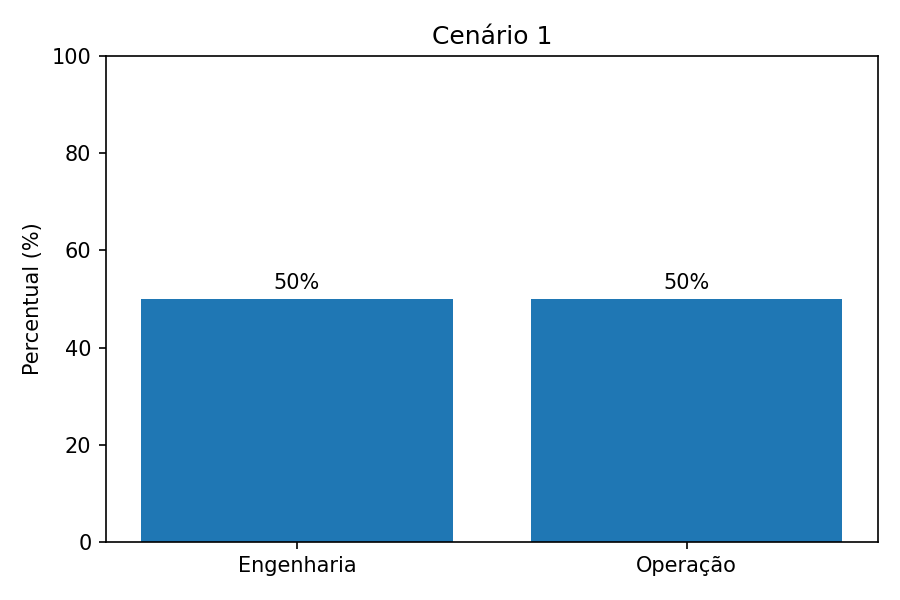
\includegraphics[width=\linewidth]{grafico_cenario_1.png}\\
    {\footnotesize 50\% Engenharia / 50\% Operação}

    \column{0.32\textwidth}
    \centering
    \textbf{Alta Automação}\\[0.2cm]
    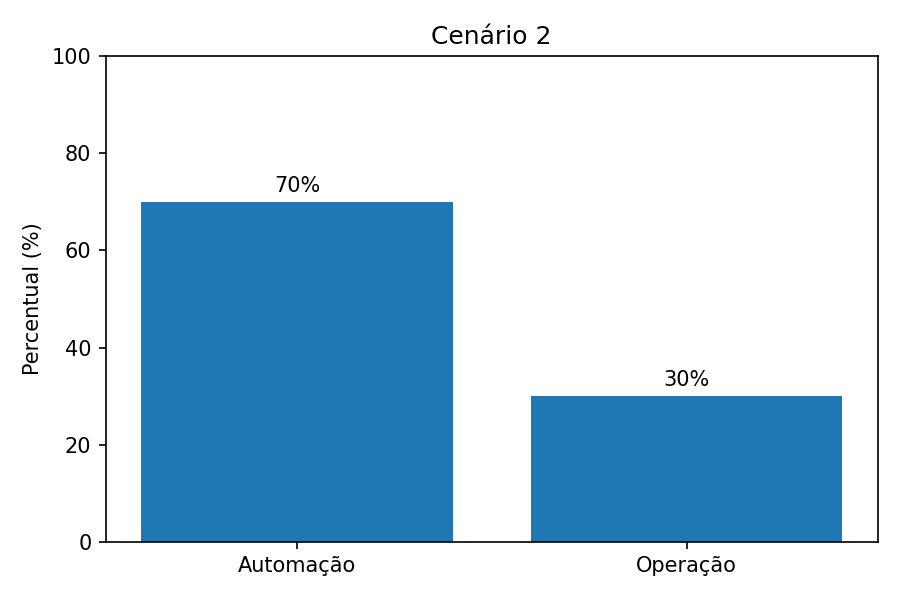
\includegraphics[width=\linewidth]{grafico_cenario_2.png}\\
    {\footnotesize 70\% Engenharia / 30\% Operação}

    \column{0.32\textwidth}
    \centering
    \textbf{Sobrecarga Operacional}\\[0.2cm]
    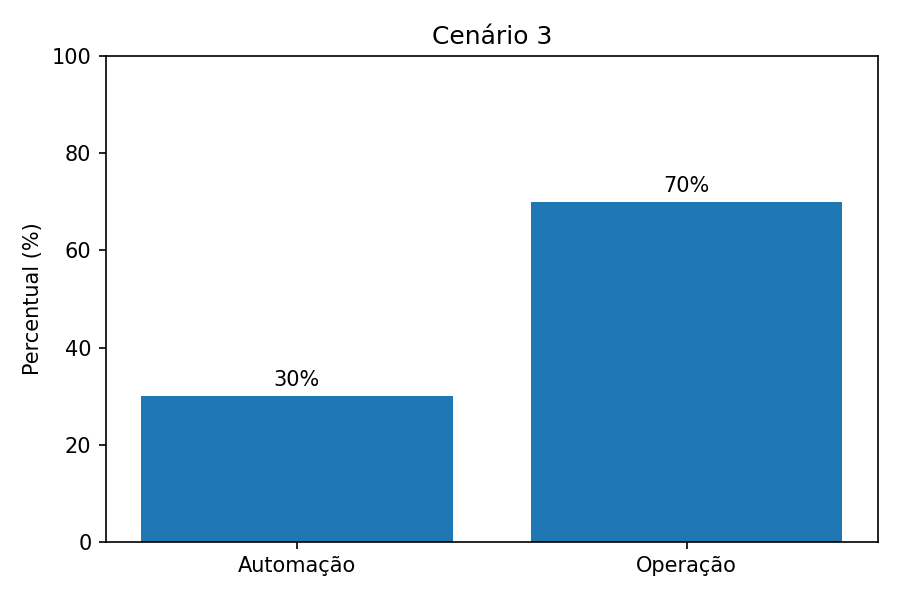
\includegraphics[width=\linewidth]{grafico_cenario_3.png}\\
    {\footnotesize 30\% Engenharia / 70\% Operação}
\end{columns}

\vspace{0.3cm}
{\scriptsize Fonte: Práticas de SRE — Google}

\end{frame}

\begin{frame}{Benefícios e Desafios do Modelo SRE}

\textbf{Principais benefícios:}
\begin{itemize}
  \item Menor custo operacional em larga escala;
  \item Sistemas que escalam com menos pessoas;
  \item Alta aceitação de mudanças e inovação contínua;
  \item Treinamento cruzado entre SRE e desenvolvimento.
\end{itemize}
 
\medskip
\textbf{Principais desafios:}
\begin{itemize}
  \item Dificuldade em contratar SREs qualificados;
  \item Necessidade de forte apoio da gerência;
  \item Decisões impopulares, como congelar lançamentos
  quando o \textit{error budget} é consumido.
\end{itemize}

\end{frame}
\begin{frame}{DevOps \textit{versus} Site Reliability Engineering (SRE)}

\begin{columns}[T]
    \column{0.48\textwidth}
    \textbf{DevOps}
    \begin{itemize}
        \item Cultura e conjunto de práticas;
        \item Foco na colaboração entre \textit{Dev} e \textit{Ops};
        \item Ênfase em automação de deploy e integração contínua;
        \item Objetivo principal: \textbf{entrega rápida de software};
        \item Métricas variáveis e pouco formalizadas;
        \item Abordagem mais filosófica do que prescritiva.
    \end{itemize}

    \column{0.48\textwidth}
    \textbf{SRE (Google)}
    \begin{itemize}
        \item Disciplina de engenharia formal;
        \item Operação de sistemas via código;
        \item Uso explícito de SLI, SLO e \textit{Error Budget};
        \item Objetivo principal: \textbf{confiabilidade com escala};
        \item Limite de 50\% do tempo em tarefas operacionais;
        \item Modelo organizacional bem definido.
    \end{itemize}
\end{columns}

\vspace{0.3cm}
\centering
{\scriptsize SRE pode ser visto como uma implementação concreta dos princípios DevOps}

\end{frame}
\begin{frame}{Princípios Fundamentais da SRE}

Embora os fluxos de trabalho variem entre equipes, todas as equipes de
\textit{Site Reliability Engineering} compartilham princípios essenciais.

\begin{itemize}
    \item Responsabilidade direta pelo serviço;
    \item Foco em confiabilidade mensurável;
    \item Ênfase em engenharia em vez de operação manual;
    \item Interação estruturada com desenvolvimento, testes e usuários.
\end{itemize}

As práticas de SRE visam garantir a operação sustentável de sistemas em
larga escala.

\end{frame}
\begin{frame}{Responsabilidades de uma Equipe de SRE}

Uma equipe de SRE é responsável por atributos críticos do serviço:

\begin{itemize}
    \item Disponibilidade e latência;
    \item Desempenho e eficiência;
    \item Gerenciamento de mudanças;
    \item Monitoração e resposta a incidentes;
    \item Planejamento de capacidade.
\end{itemize}

Essas responsabilidades são exercidas por meio de código, automação
e métricas objetivas.

\end{frame}
\begin{frame}{Garantindo um Foco Durável em Engenharia}

O Google impõe um limite claro:
\begin{itemize}
    \item Máximo de \textbf{50\% do tempo} em tarefas operacionais;
    \item Pelo menos \textbf{50\% do tempo} em desenvolvimento e engenharia.
\end{itemize}

Quando esse limite é ultrapassado:
\begin{itemize}
    \item Tarefas operacionais são devolvidas ao time de desenvolvimento;
    \item Desenvolvedores participam de plantões;
    \item O sistema recebe feedback para reduzir intervenção manual.
\end{itemize}

Esse mecanismo atua como uma \textit{válvula de segurança organizacional}.

\end{frame}
\begin{frame}{Incidentes, Plantão e Cultura de Postmortem}

Diretrizes operacionais da SRE:
\begin{itemize}
    \item Ideal: até \textbf{2 incidentes} por turno de plantão (8–12h);
    \item Excesso de alertas indica falhas estruturais no sistema;
    \item Postmortems devem ser escritos para todos os incidentes relevantes.
\end{itemize}

O Google adota uma cultura de:
\begin{itemize}
    \item Postmortems sem culpabilização;
    \item Identificação de causas-raiz;
    \item Ações corretivas baseadas em engenharia.
\end{itemize}

\end{frame}


\end{document}
